\chapter{Methods\label{chap:methods}}

Image processing and CIV analysis were conducted in self-written Python code using the following libraries: Astropy, Matplotlib, NumPy, Pandas, NetCDF4, and Skimage.

\section{Image Processing}

Since Cross-Correlation Image Velocimetry (CIV) relies on detecting moving features in image sequences, the aim is to enhance cloud visibility by improving image contrast. This approach is intended to make clouds more distinguishable and facilitate more accurate cloud tracking. To achieve this, four spatial domain image processing methods were selected for comparison: histogram matching, histogram equalization (HE), contrast limited adaptive histogram equalization (CLAHE), and sigmoid transformation. Other methods such as histogram slicing and stretching were avoided because they would have resulted in the loss of certain pixel intensities while the chosen methods preserve all data.

\subsection{Histogram Matching}

Given the slight variations in brightness observed among the image sequences, histogram matching, was applied. The goal was to achieve consistent brightness across all images within a sequence, thereby improving the similarity of pixel intensities for moving features and reducing the impact of variations in solar illumination.

Histogram matching is used to generate images, that have a specified histogram. It was implemented in this thesis using the skimage package in Python. The steps include the computation of the source image’s cumulative distribution function (CDF) and the target image’s CDF, which are used to determine a mapping function\cite{Gonzalez2018}. This function maps each intensity in the source image by finding the intensity in the target image that is closest to the corresponding value in the CDF of the source image. 

Since the CDF is derived from the PDF, the probability density function is given by\cite{Gonzalez2018}: 

\begin{equation}
p(r_k) = \frac{n_k}{N}
\end{equation}

where \( n_k\) is the amount of intensity values \( r_k \) and \(N\) the total number of pixels in the image, while \( p(r_k)\) is the probability of an intensity occurring at \( r_k \).

The cumulative distribution function is the running total of the probabilities from the PDF at each step, given by\cite{Gonzalez2018}: 

\begin{equation}
c(r_i) = \frac{1}{N} \sum_{j=0}^{r_i} n_j
\end{equation}

where \( r_i\) is the intensity level for which the CDF is calculated, \( n_j\) is the amount of intensities \( j\), \(N\) the total number of pixels and \(c(r_i)\) the cumulative probability up to the specified intensity \( r_i\). 

The pixel intensity mapping is given by\cite{Gonzalez2018}: 

\begin{equation}
s_i = \text{round} \left( \text{c}_{\text{target}}^{-1} \left( \text{c}_{\text{source}}(r_i) \right) \right)
\end{equation}

where \( s_i\) is the updated pixel intensity, \( r_i\) is the original intensity, \(\text{c}_{\text{target}}^{-1}\) is the inverse CDF of the target histogram, \(\text{c}_{\text{source}}(r_i)\) is the CDF of the source histogram at the intensity \( r_i\). The result is rounded to the nearest integer to enable mapping to the closest intensity, which wouldn't be possible with discrete values.  

For the selected sequences, the first image in each sequence served as the reference, and subsequent were adjusted based on the CDF of the reference. 
\FloatBarrier
\begin{figure}[h!] 
    \centering
    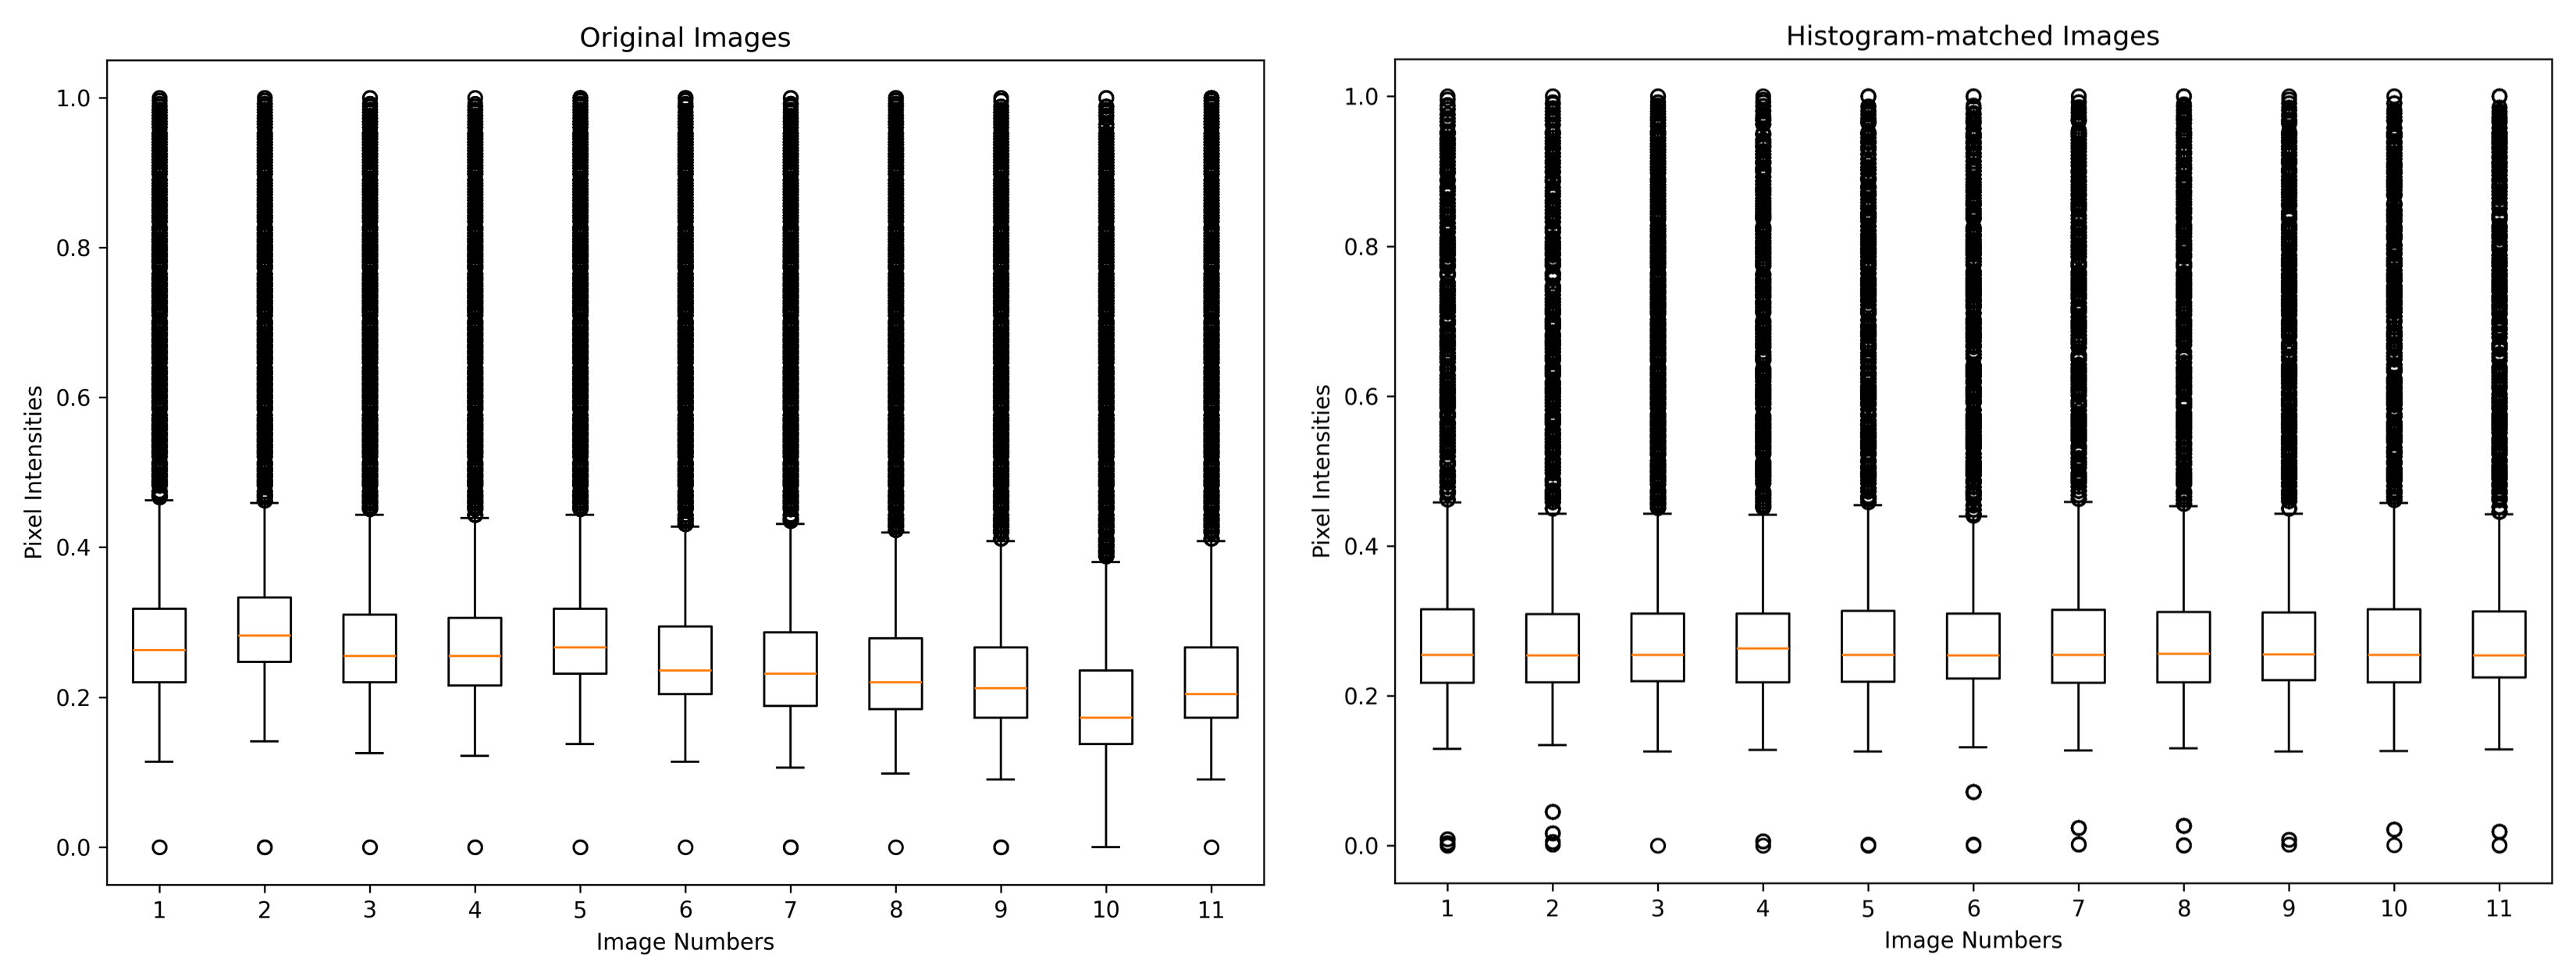
\includegraphics[width=1\textwidth]{fig_20.png}
    \caption{Box plot of the image sequence from UTC: 24/12/2021 10:30:07 - 11:20:06 before histogram matching on the left and after histogram matching on the right.}
\end{figure}
\FloatBarrier
The box plots (see Figure 3.1) and visual observation (see Figure 3.2) clearly indicate that the brightness levels within the sequences have become more consistent. 
\FloatBarrier
\begin{figure}[h!] 
    \centering
    \includegraphics[width=1\textwidth]{fig_21.png}
    \caption{Comparison of raw and histogram-matched images (UTC: 24/12/2021, 11:15:06 - 11:20:06). Upon closer inspection, the raw image on the left appears darker compared to the one on the right. The histogram-matched images below exhibit more consistent brightness levels.}
\end{figure}
\FloatBarrier
\subsection{Histogram Equalization}

Histogram equalization is widely used for contrast manipulation, readjusting the original histogram to produce a uniform population density of pixels\cite{Ghosh2013}. It makes both darker and lighter areas of the image more visible, improving the overall contrast.
The processing steps are similar to the ones for histogram matching. The only difference is the mapping function used, given by\cite{Gonzalez2018}: 

\begin{equation}
s_i = \text{round} \left((L-1) \cdot c(r_i) \right)
\end{equation}

where \( s_i\) is the updated intensity, \( L\) is the number of possible intensity levels and \( c(r_i)\) the CDF of the intensity at \( r_i\).
\FloatBarrier
\begin{figure}[h!] 
    \centering
    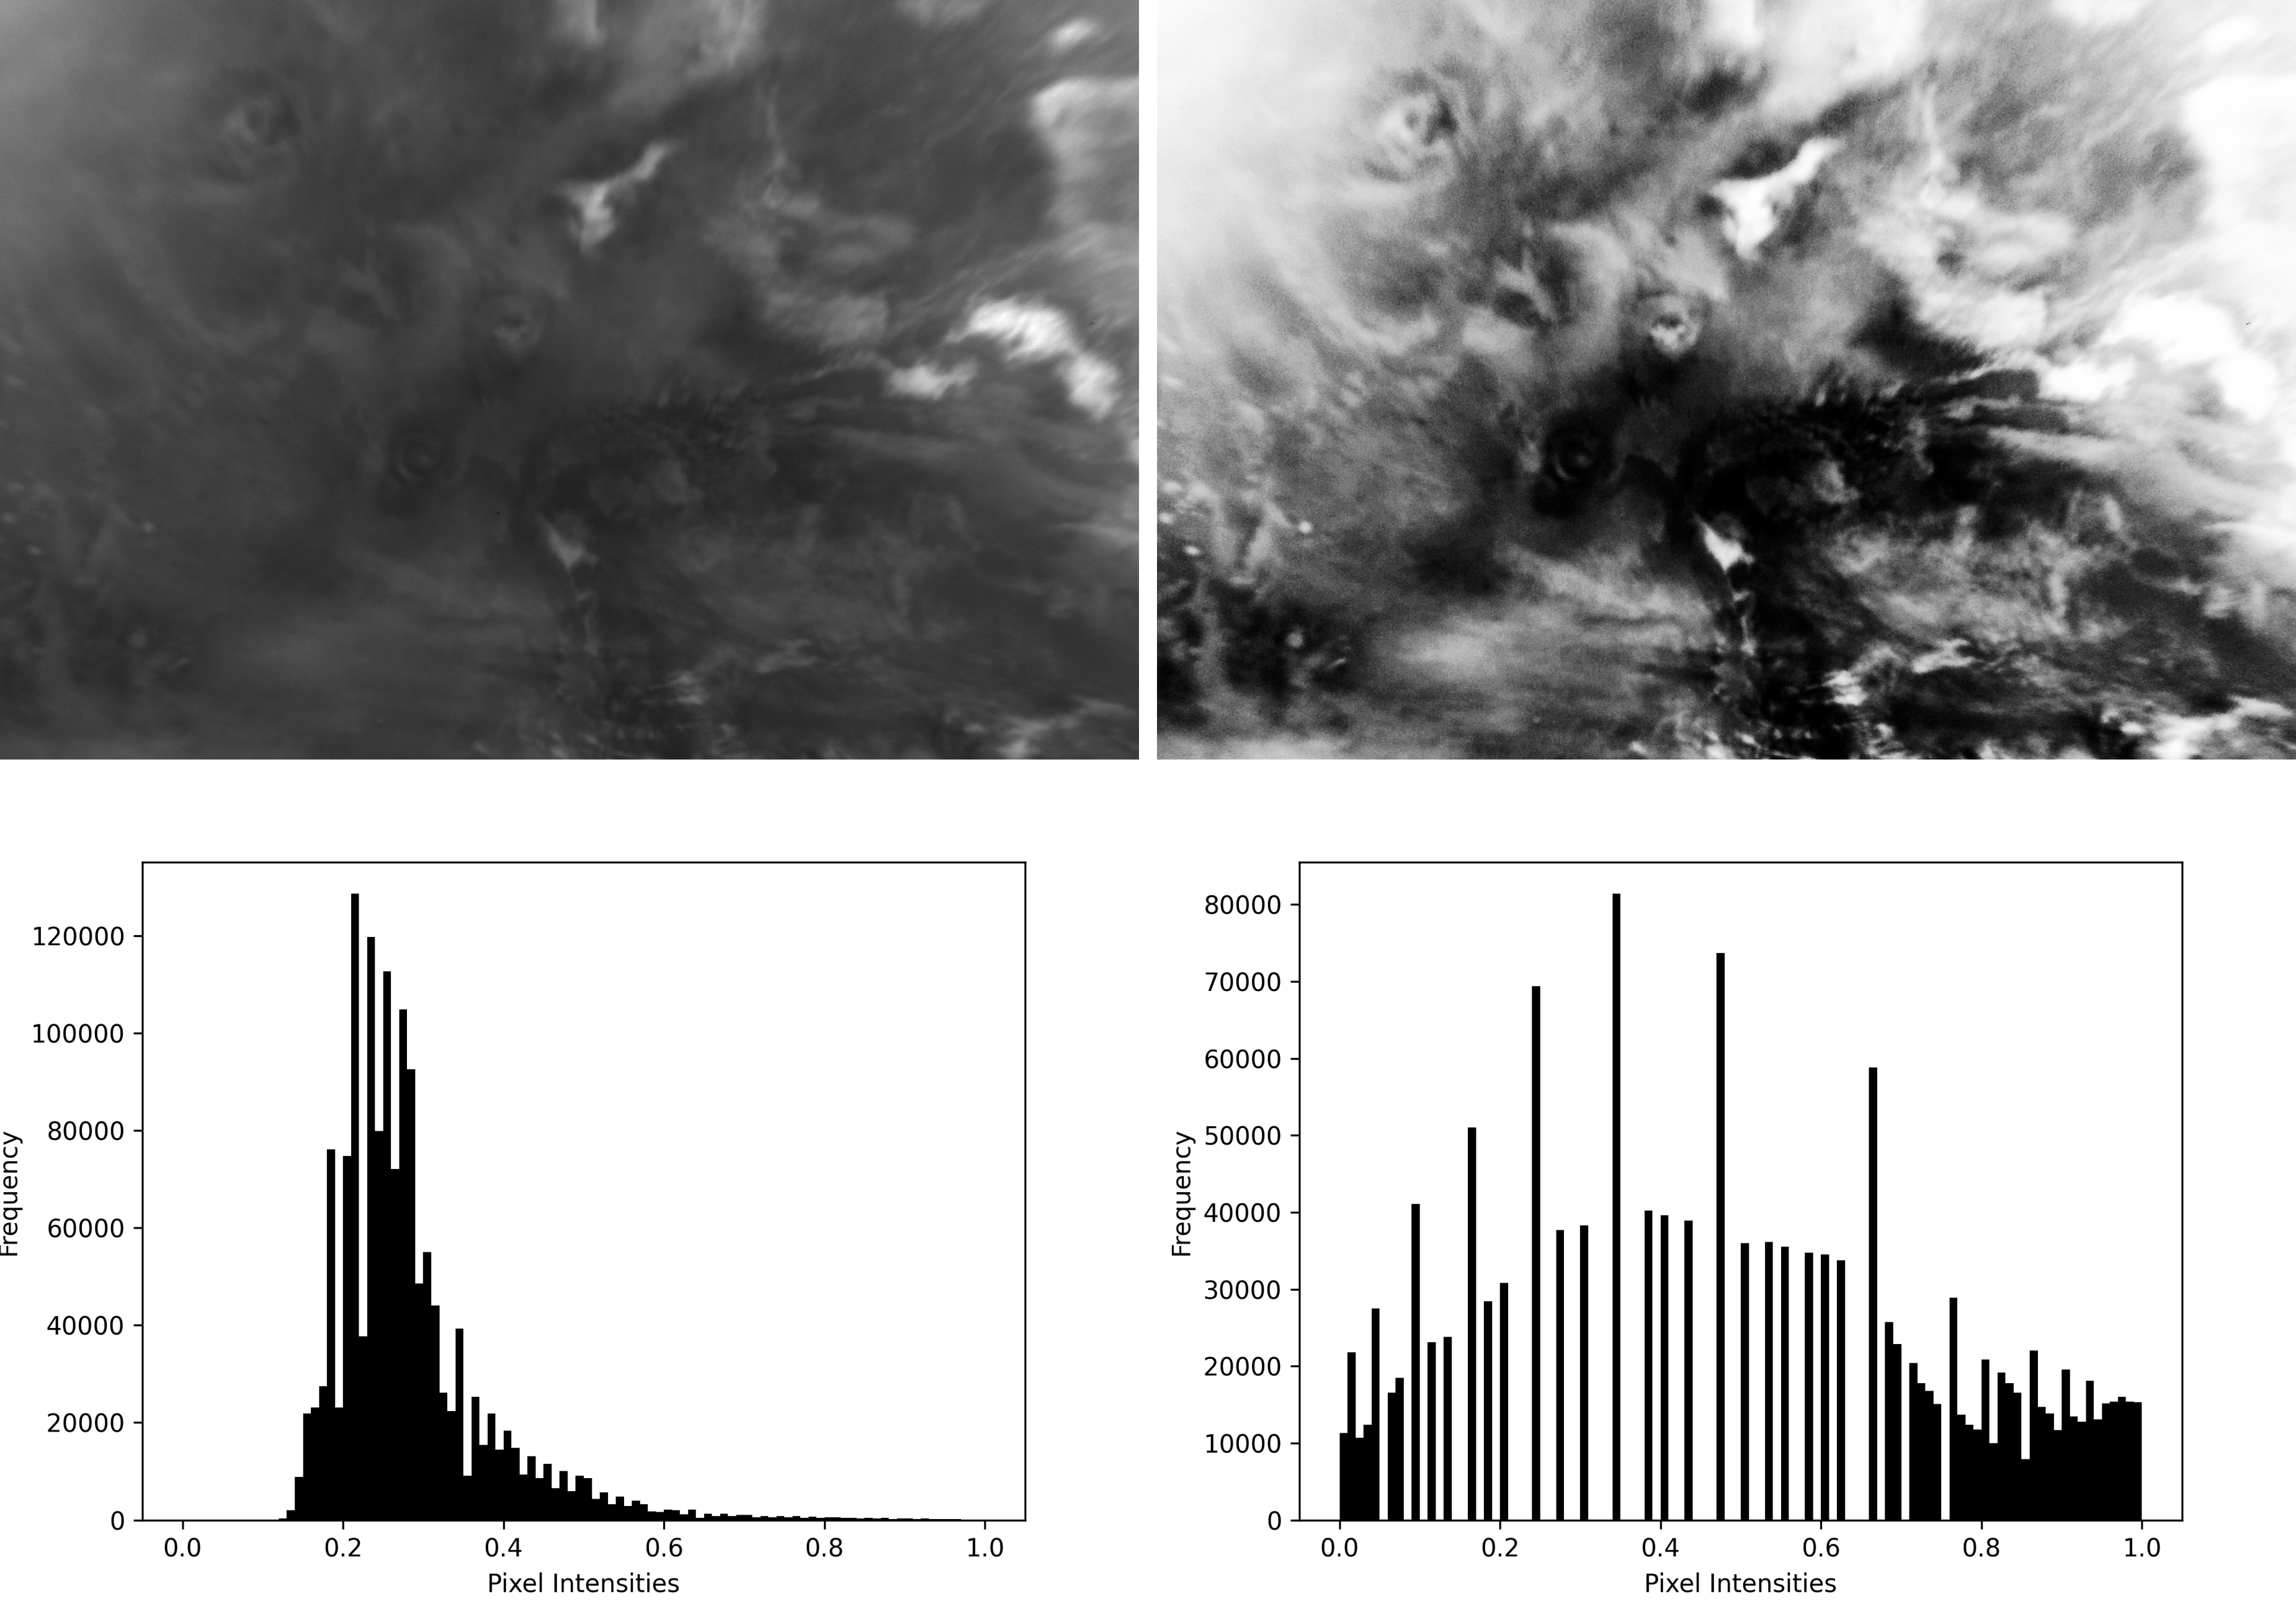
\includegraphics[width=1\textwidth]{fig_22.png}
    \caption{Comparison of raw and histogram-equalized image (UTC: 24/12/2021, 10:30:07). The original image including the intensity histogram are on the left, while the histogram-equalized image and the intensity histogram are on the right.}
\end{figure}
\FloatBarrier
The images exhibit higher contrast (as shown in Figure 3.3). Comparing the image histograms before and after HE, the pixel intensities are more evenly distributed across the intensity range.

\subsection{Contrast Limited Adaptive Histogram Equalization}

Adaptive Histogram Equalization is another technique for improving image contrast. It differs to histogram equalization in that for every pixel at position \( (i,j)\) in the image, the CDF is calculated for a filter window centered on that pixel, where the filter window size is defined before-hand and the window moves pixel-wise from left to right\cite{Haertinger2024}. It potentially maps a narrow range of input values to a wide range of output values if the window size encompasses a homogeneous image region. Histogram clipping, used in CLAHE, addresses this issue by reducing the amount of contrast enhancement by limiting histogram bins to a clip limit.

In this thesis, the clip limit was set to 0.1, hence intensity values in uniform regions of the image are not increased by more than 0.1. Thereby, the contrast enhancement remains moderate, preventing excessive stretching. The kernel size was set to 100x100 pixels based on the pixel sizes of the clouds.
\FloatBarrier
\begin{figure}[h!] 
    \centering
    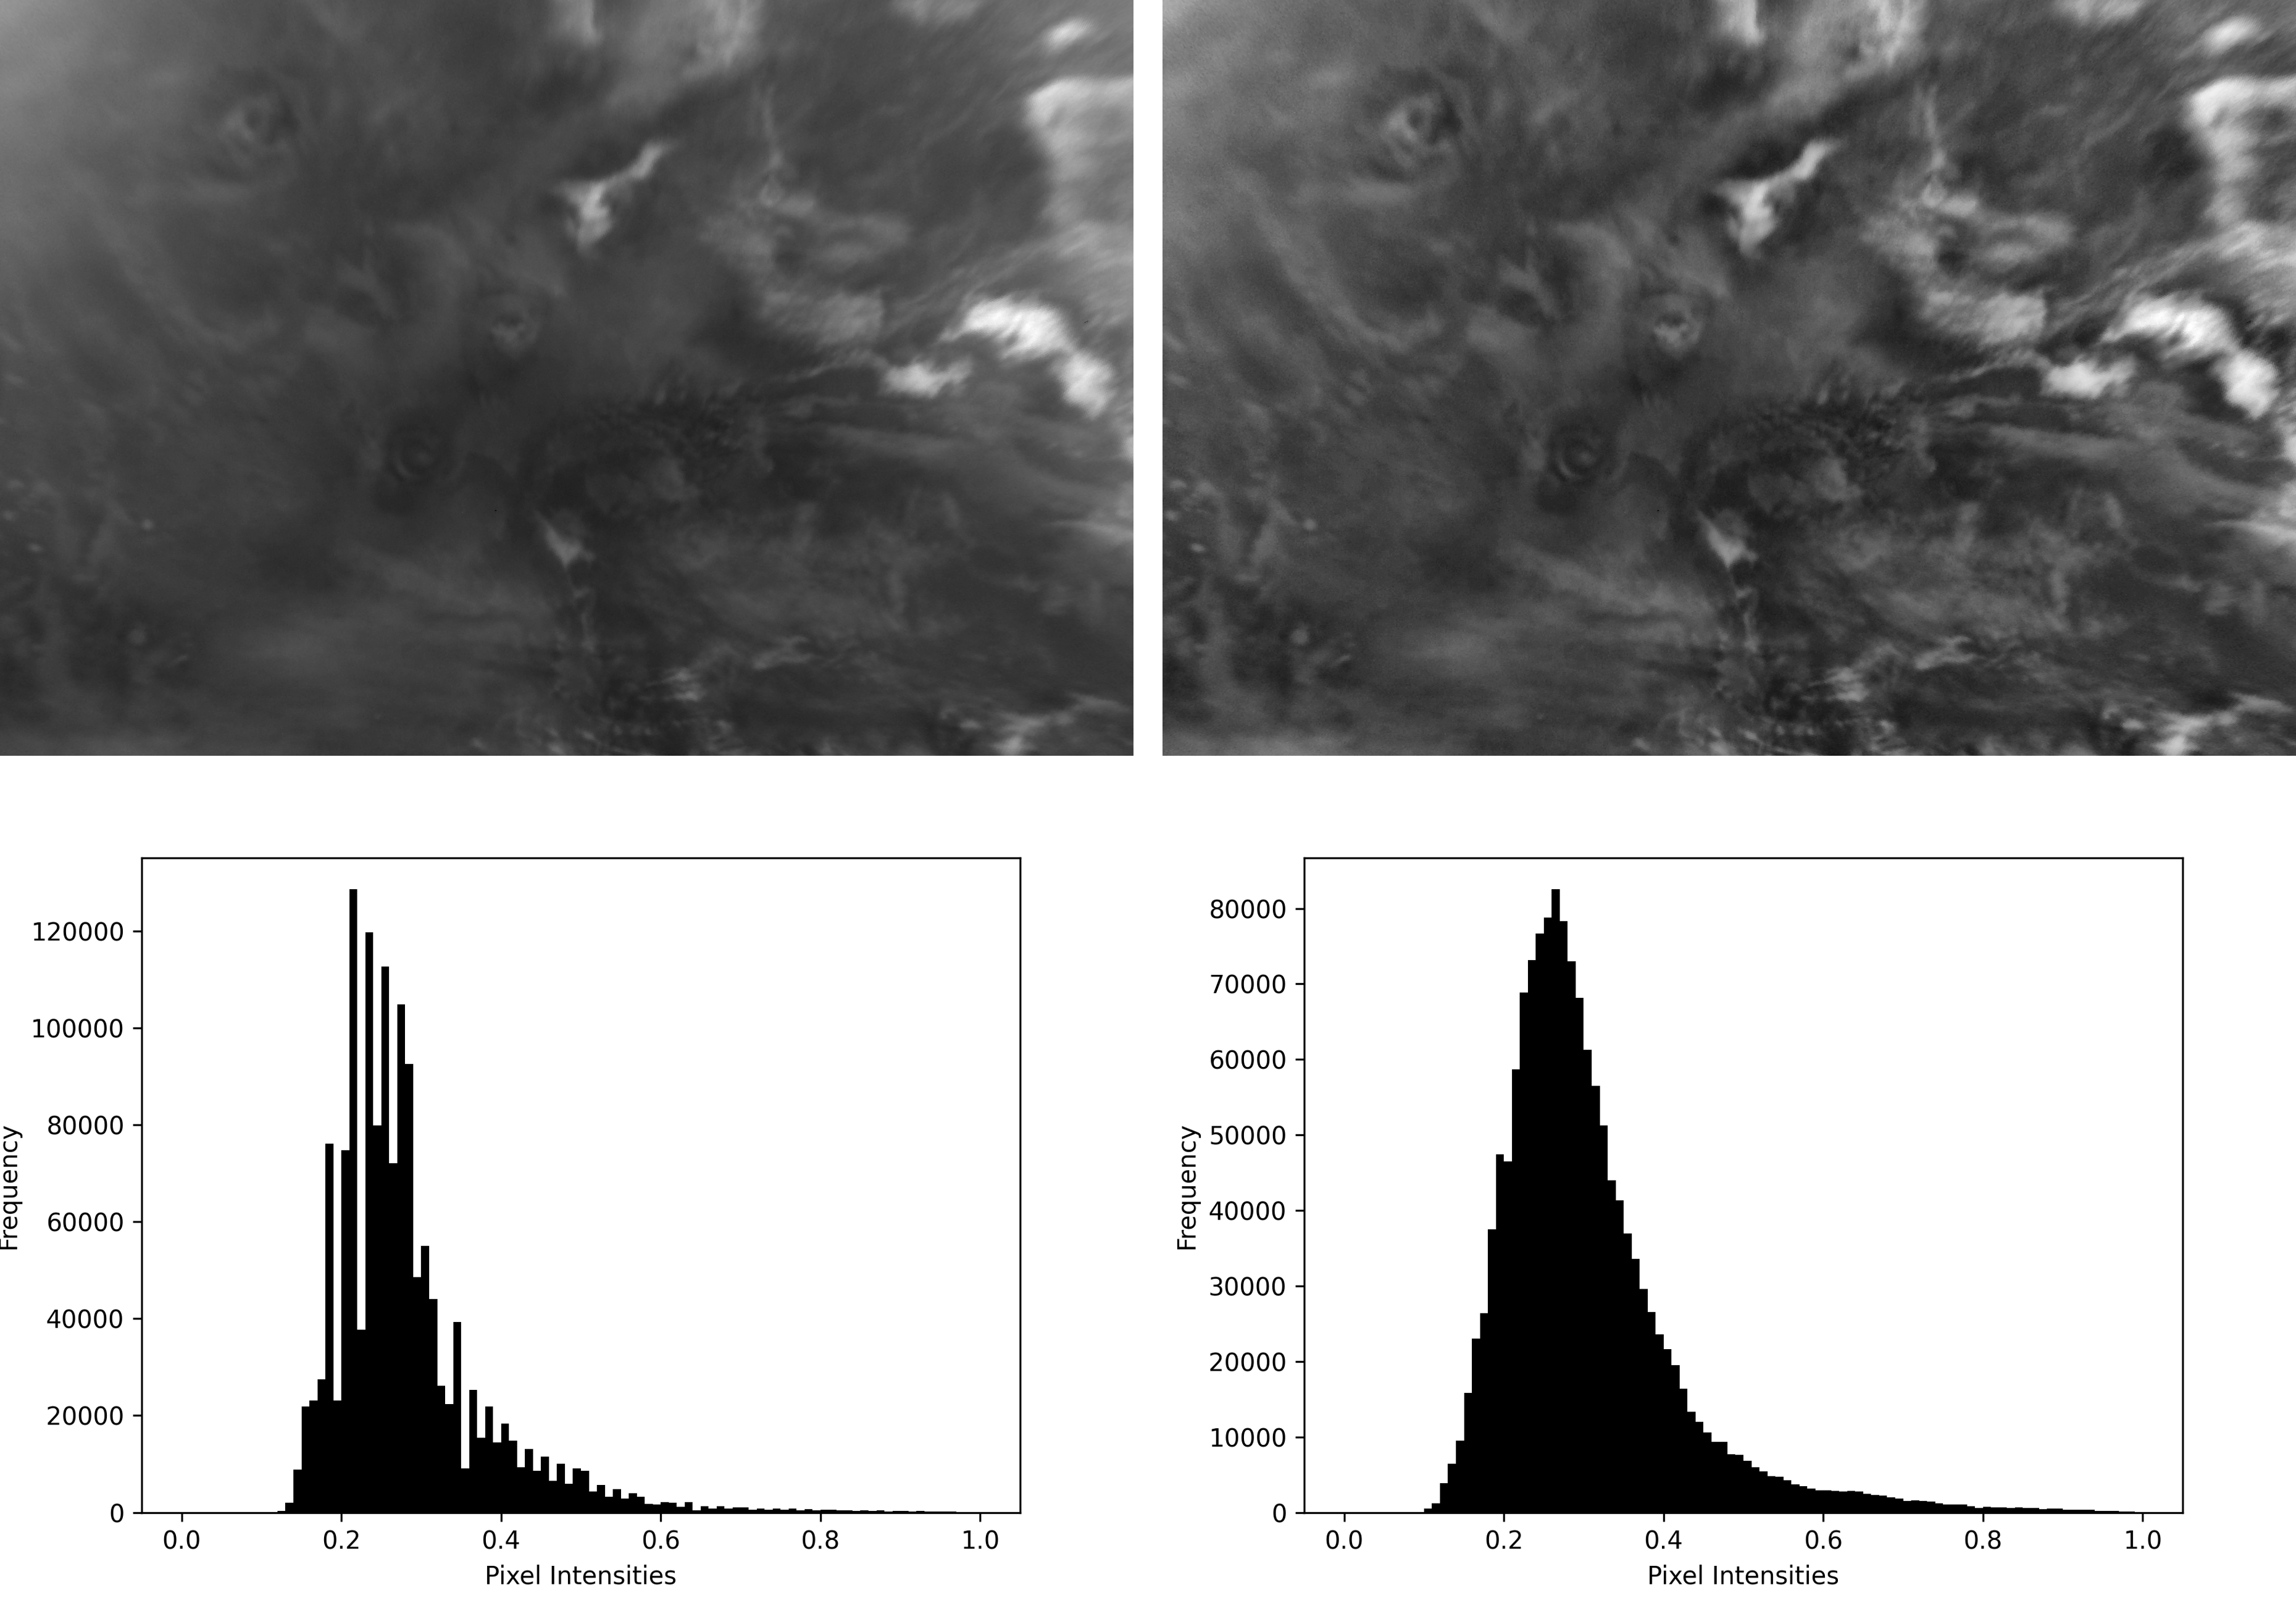
\includegraphics[width=1\textwidth]{fig_23.png}
    \caption{Comparison of raw and CLAHE-transformed image (UTC: 24/12/2021, 10:30:07). The original image including the intensity histogram are on the left, while the CLAHE-transformed image and the intensity histogram are on the right.}
\end{figure}
\FloatBarrier
The transformed images show reduced contrast compared to the histogram-equalized images (see Figure 3.4). However, clouds that were obscured in darker regions are more visible. Additionally, the histograms display smoother transitions.

\subsection{Sigmoid Transformation}

While the previous two methods involved linear transformations of the pixel data, the sigmoid transformation is a non-linear approach. Applying the sigmoid function to the pixel values can enhance details in darker regions while preserving the natural appearance of the image. The sigmoid transformation is given as follows\cite{Braun2000}: 

\begin{equation}
x_{\text{transformed}} = \frac{1}{1 + e^{-\alpha (x - \beta)}}
\end{equation}

where \( x_{\text{transformed}}\) is the transformed pixel value, \( x\) is the input value, \( \alpha\) is the cut-off factor which controls the steepness, and \( \beta\) is the gain factor that controls the midpoint of the curve. The effect of cut-off and gain factors is illustrated in Figure 3.5. 
\FloatBarrier
\begin{figure}[h!] 
    \centering
    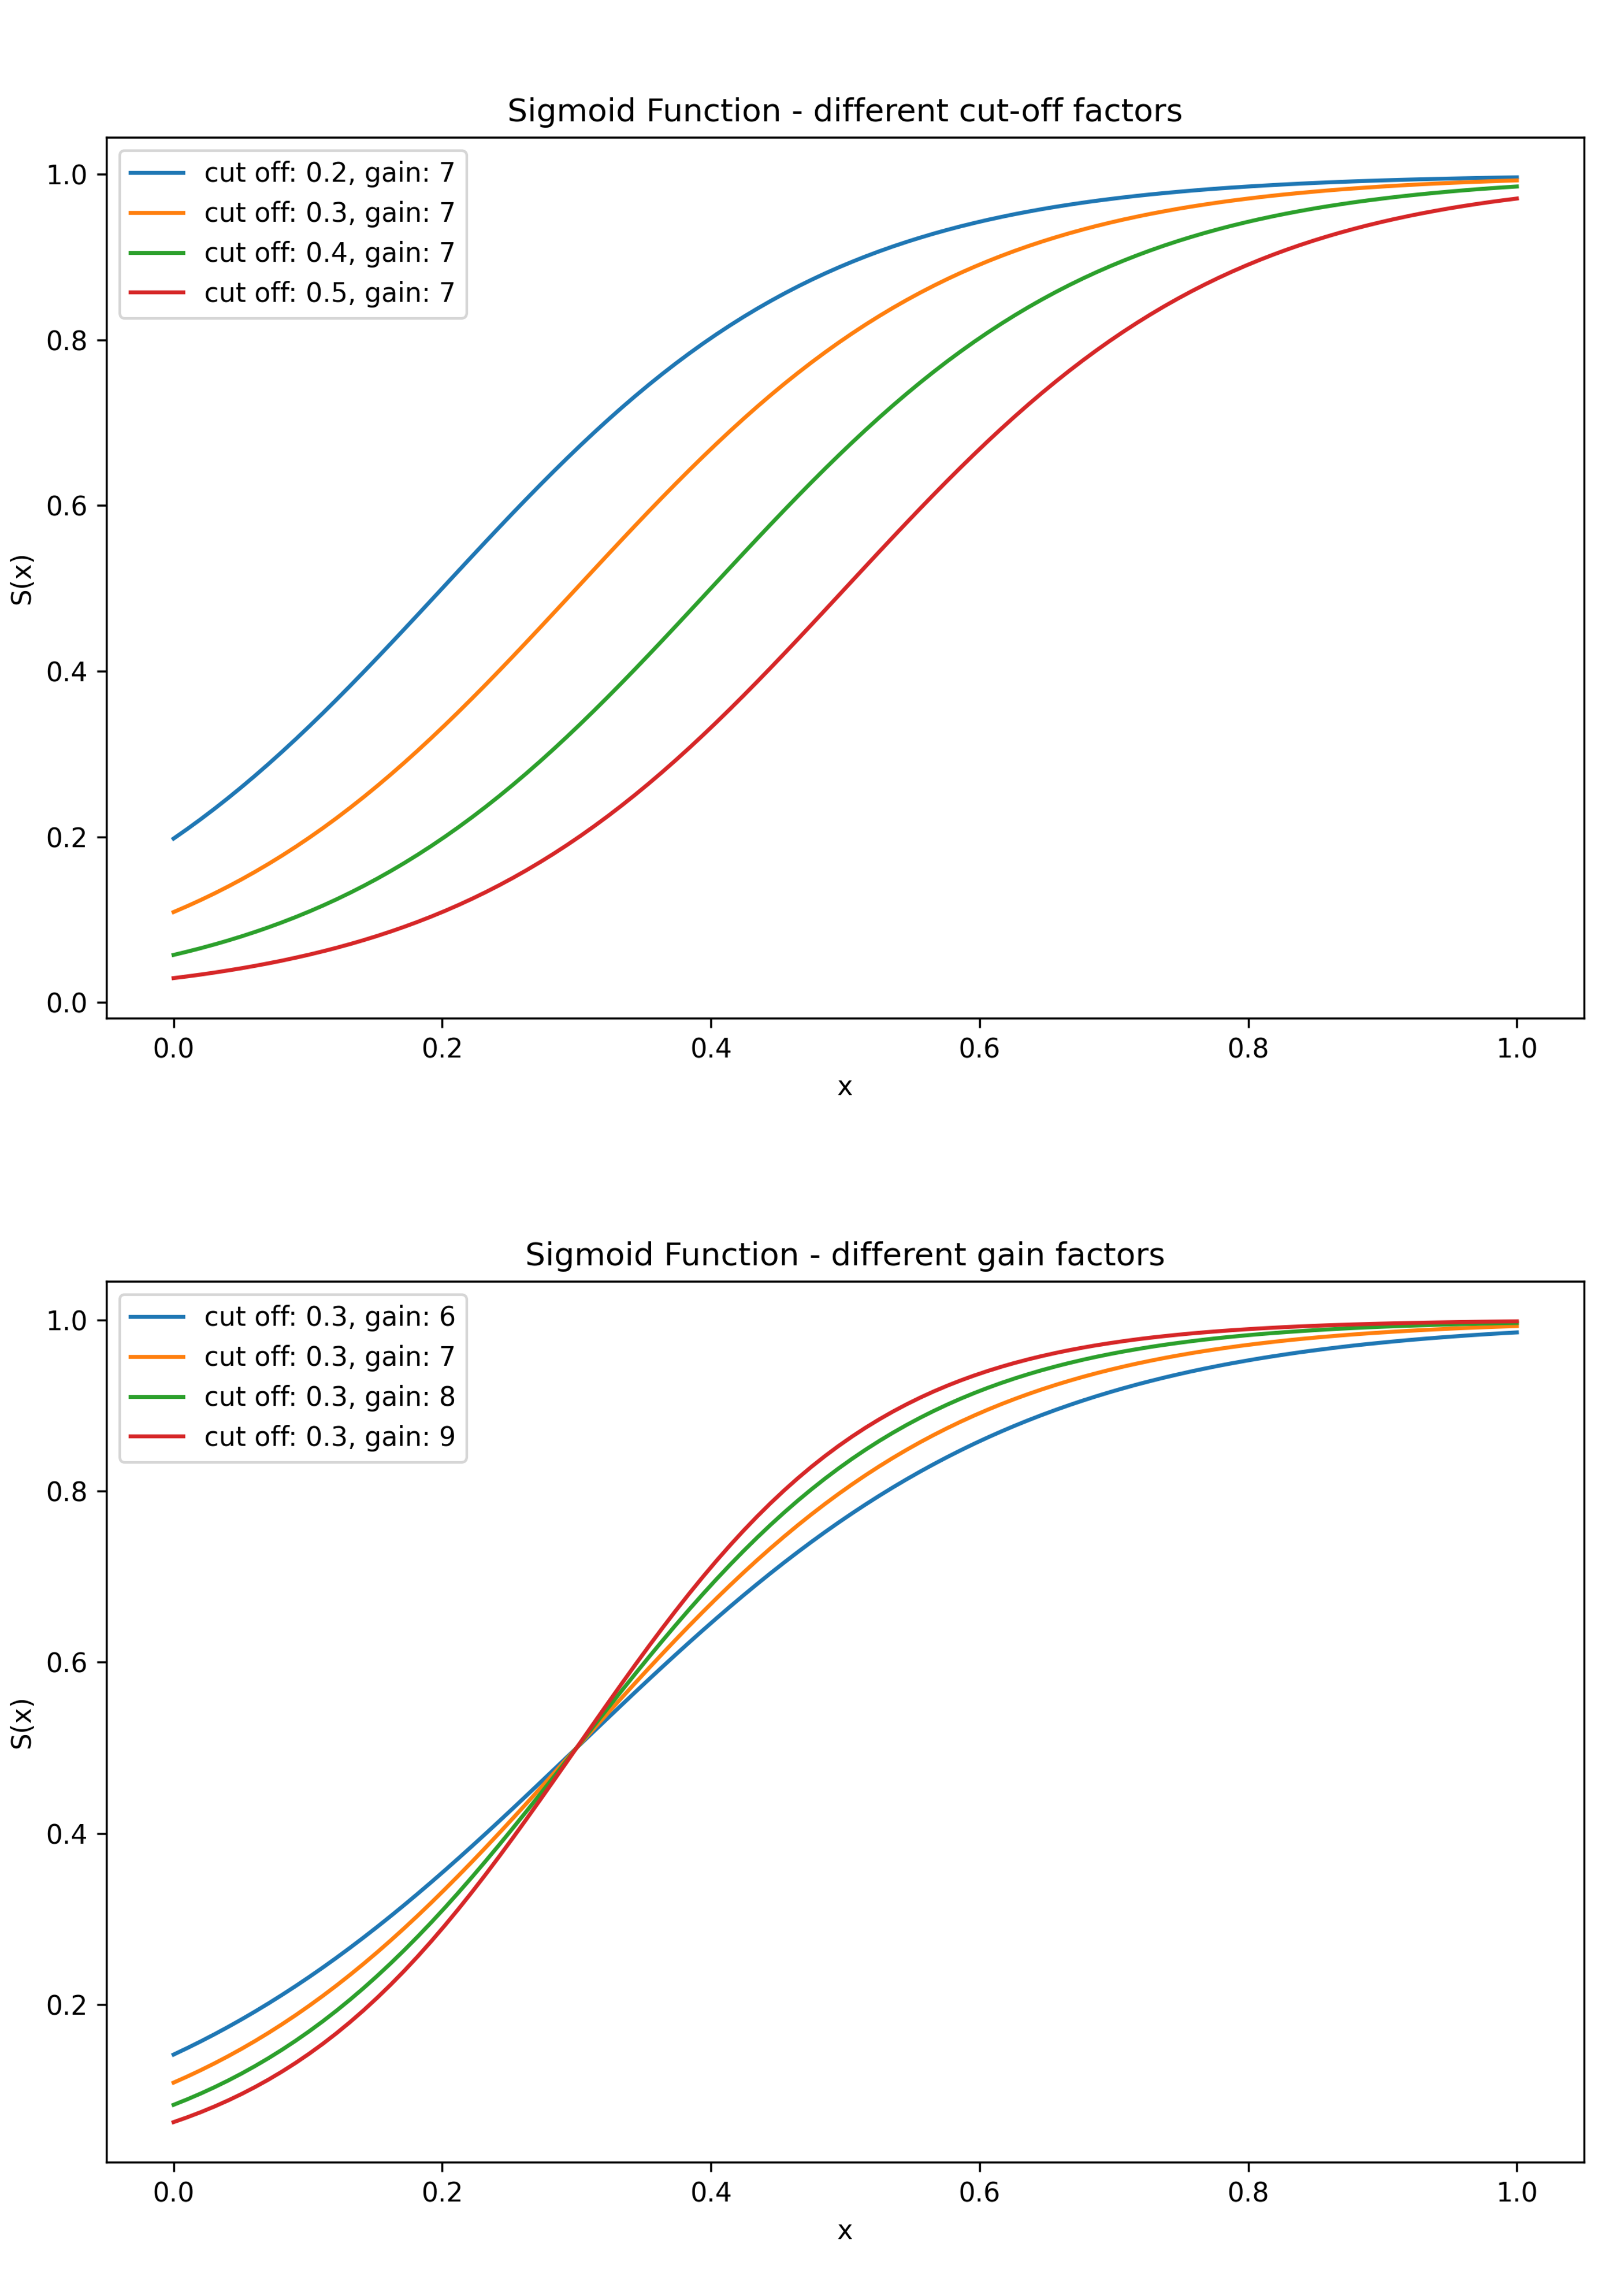
\includegraphics[width=0.8\textwidth]{fig_24.png}
    \caption{Visualisation of the sigmoid function. The plot at the top displays the function with different cut-off factors and the plot at the bottom displays the effect of changing the gain factor.}
\end{figure}
\FloatBarrier
For the given image sequences, the cut-off factor ranged between 0.3 and 0.4 and the gain factor varied between 6 and 8.
\FloatBarrier
\begin{figure}[h!] 
    \centering
    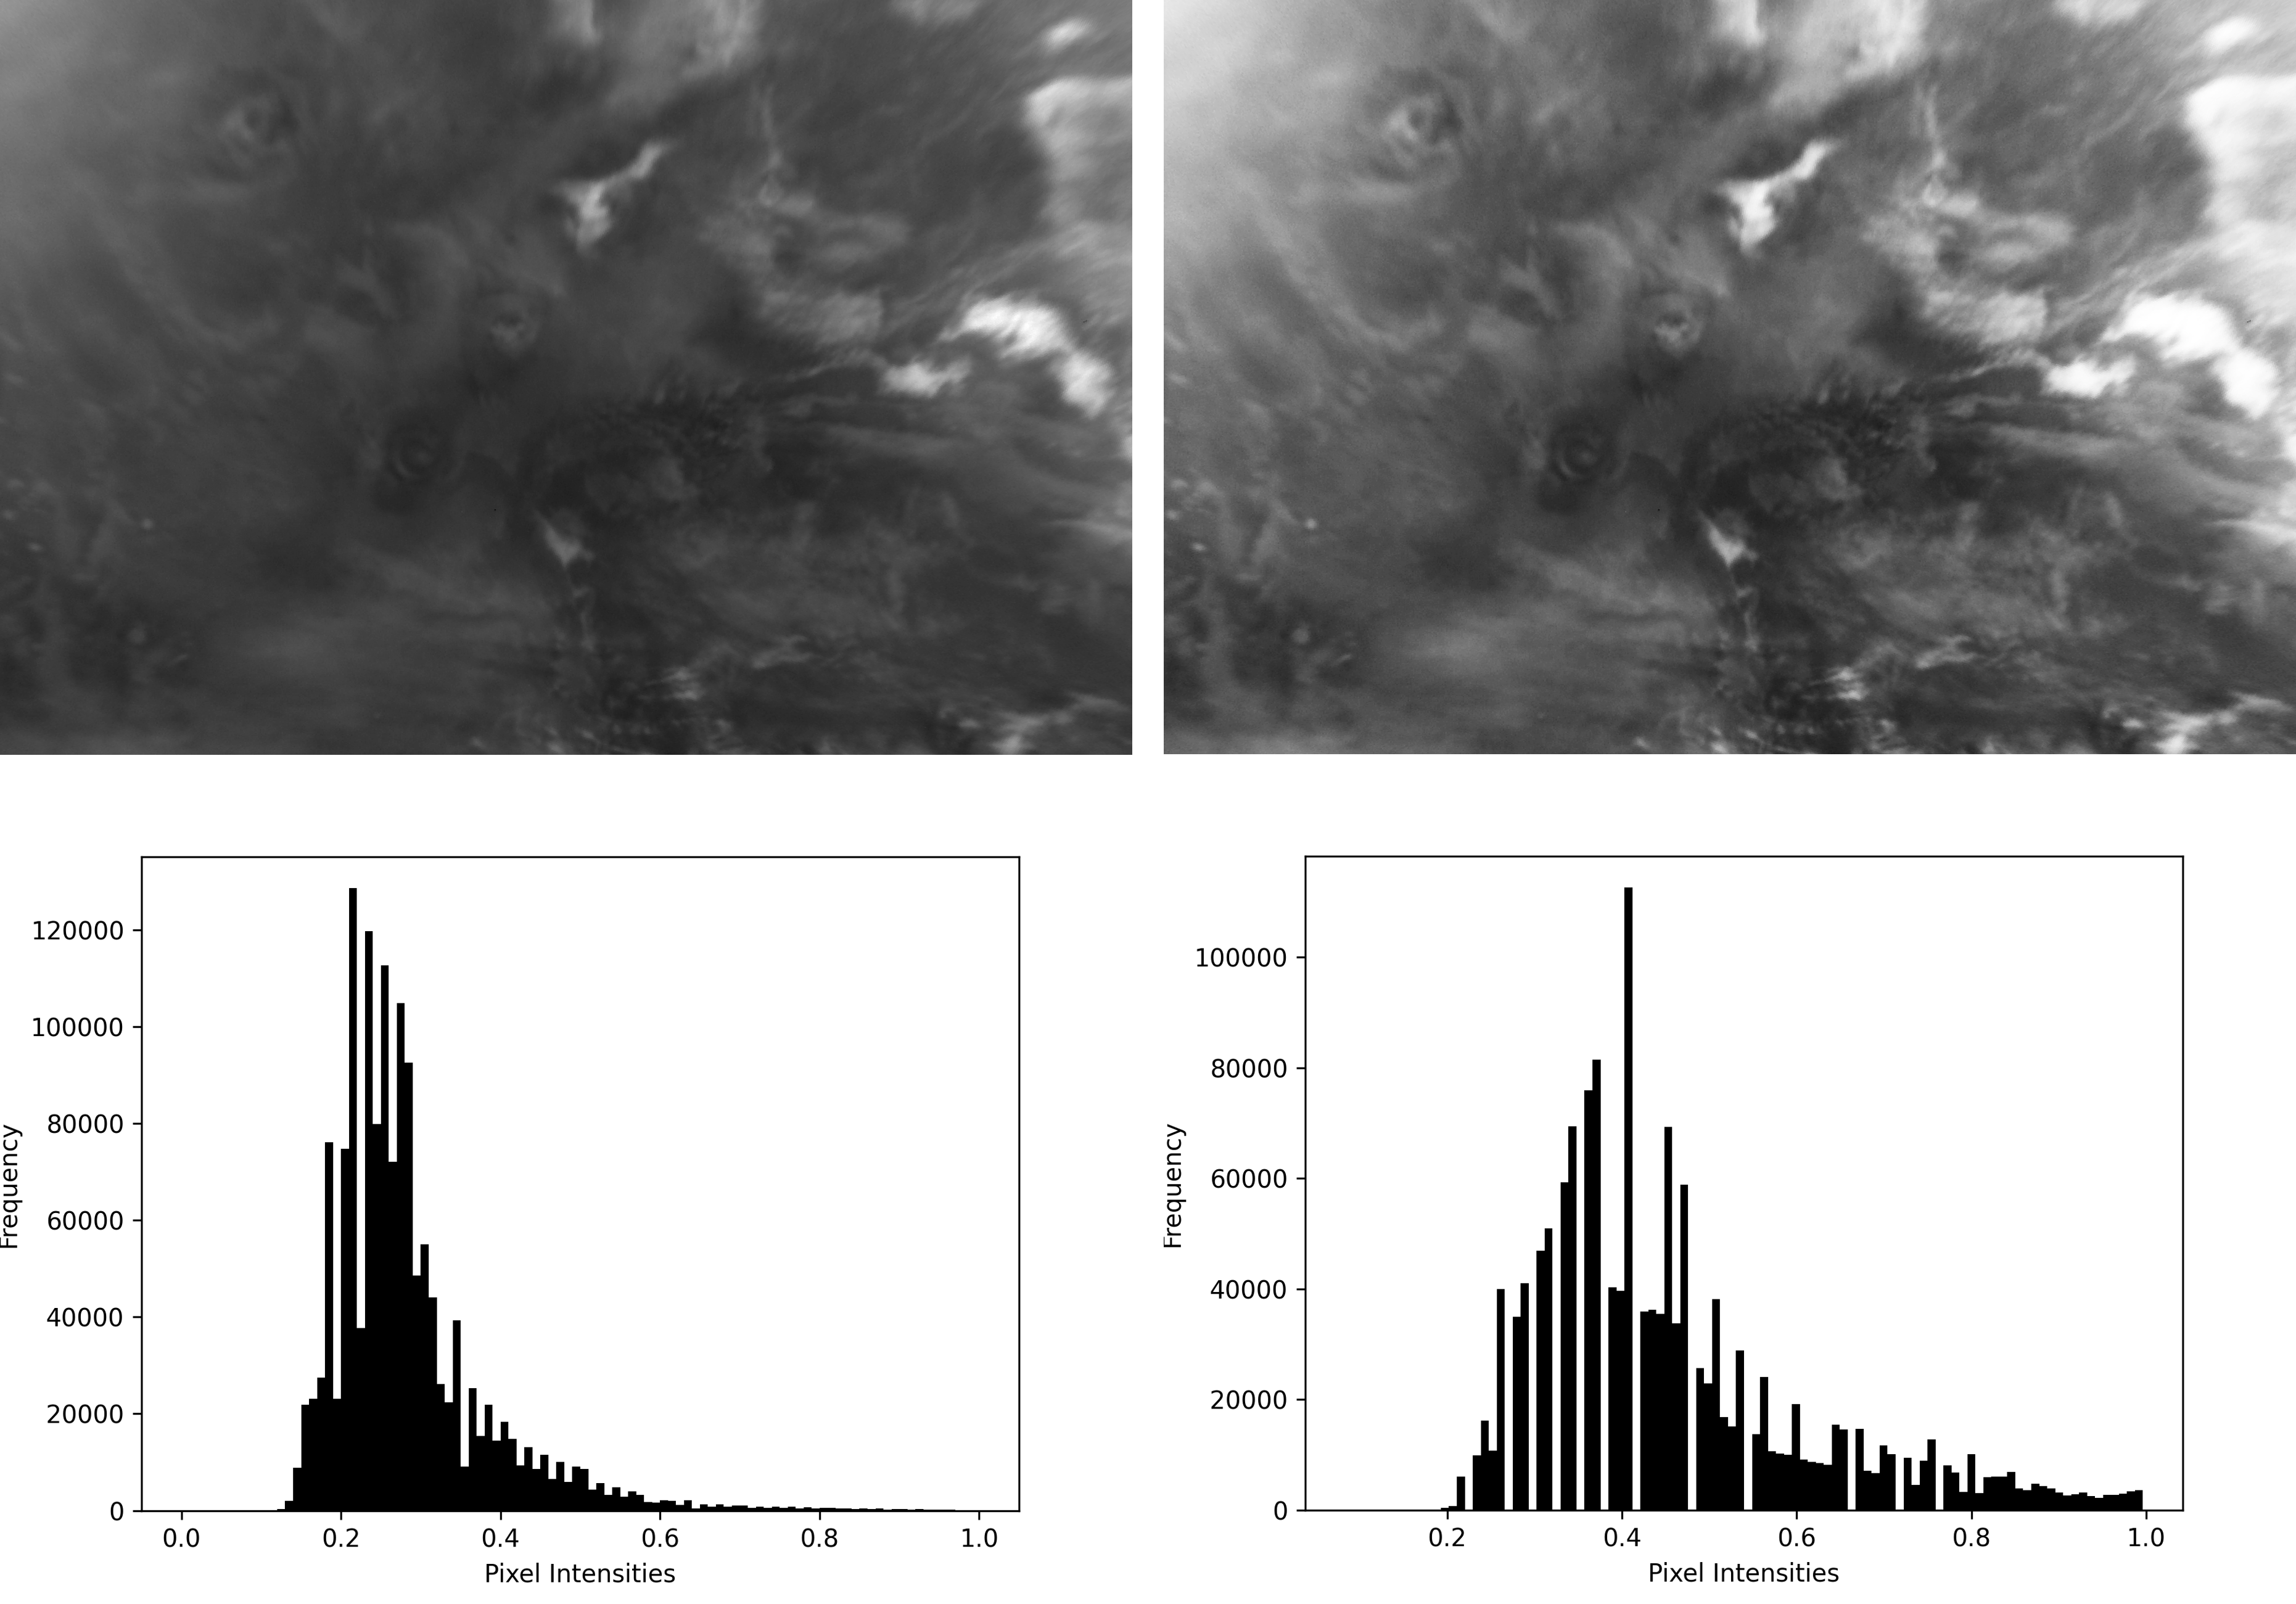
\includegraphics[width=1\textwidth]{fig_25.png}
    \caption{Comparison of raw and sigmoid-transformed image (UTC: 24/12/2021, 10:30:07) with a cut-off factor of 0.3 and a gain factor of 8. The original image including the intensity histogram are on the left, while the sigmoid-transformed image and the intensity histogram are on the right. }
\end{figure}
\FloatBarrier
The resulting images (see Figure 3.6) are brighter, but darker areas haven't been overemphasized. The clouds are more visible, and the histogram retains its shape. However, the pixel intensities are stretched and more evenly distributed.

\section{Cloud Tracking}

To track cloud movements, Correlation Image Velocimetry (CIV) was employed. CIV, a technique based on cross-correlation, was executed using UVMAT — a Matlab-based interface\cite{SoftUVMAT}. After conducting the CIV-analysis, the results were converted into velocity vectors, measured in meters per second. 

\subsection{Correlation Image Velocimetry}

CIV which is a type of Particle Image Velocimetry (PIV), is a motion tracking method. Initially used in fluid mechanics, it has also shown significant utility in tracking clouds in satellite imagery. CIV involves dividing the image into smaller segments, called interrogation windows (as illustrated in Figure 3.7). For each window, velocity vectors are computed by applying cross-correlation to pairs of images\cite{Scharnowski2020} (as shown in Figure 3.8).
\FloatBarrier
\begin{figure}[h!] 
    \centering
    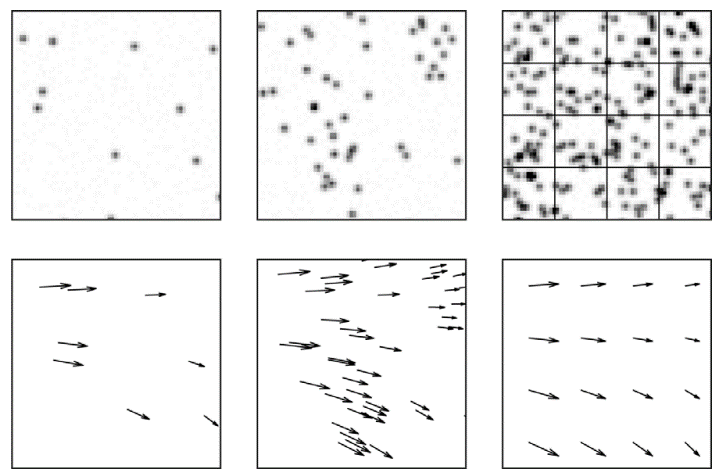
\includegraphics[width=0.7\textwidth]{fig_26.png}
    \caption{Concept visualisation of tracking individual particle images at low (left) and medium (center) density and correlating interrogation windows (right)\cite{Scharnowski2020}. While the images at the top show the particle image distribution, the bottom images display the resulting displacement fields.}
\end{figure}
\FloatBarrier
\begin{figure}[h!] 
    \centering
    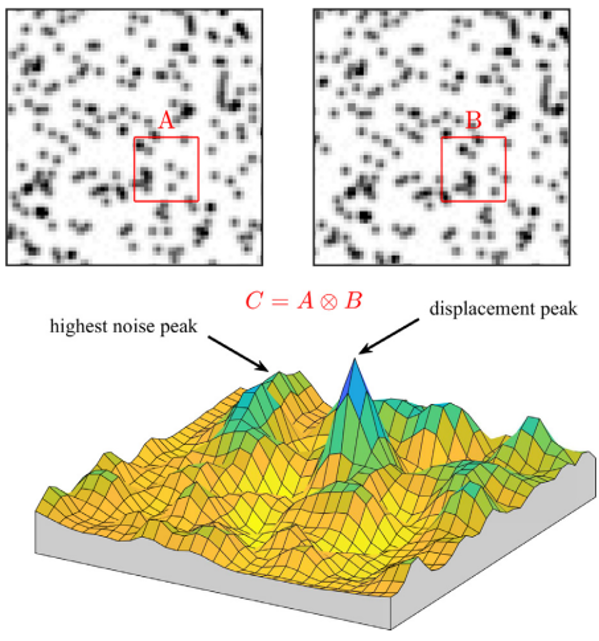
\includegraphics[width=0.7\textwidth]{fig_27.png}
    \caption{Illustration of the cross-correlation process: This example shows a pair of PIV images, capturing the particle distribution at two different times\cite{Scharnowski2020}. The red boxes, each measuring 16 x 16 pixels, highlight the interrogation windows A and B. The bottom image displays the resulting cross-correlation function, where a distinct peak indicates the displacement of the particle images.}
\end{figure}
\FloatBarrier
Using the UVMAT-interface (see Figure 3.9), the images were processed through a six-step process: CIV1, FIX1, PATCH1, CIV2, FIX2, and PATCH2\cite{SoftUVMAT}. 

In the CIV1 stage, initial CIV is performed based on the specified interrogation window and shift box size, where the latter defines the area within which CIV is allowed to detect movements, while the grid size determines the number of vectors displayed. The FIX1 stage corrects errors and filters vectors above a pre-defined correlation co-efficient. PATCH1 applies a smoothness filter using interpolation and determines the maximum vector size. 
CIV2, FIX2 and PATCH2 repeat the process using vectors obtained from CIV1, additionally allowing for refined parameter adjustments and accounting for rotation and deformation.
\FloatBarrier
\begin{figure}[h!] 
    \centering
    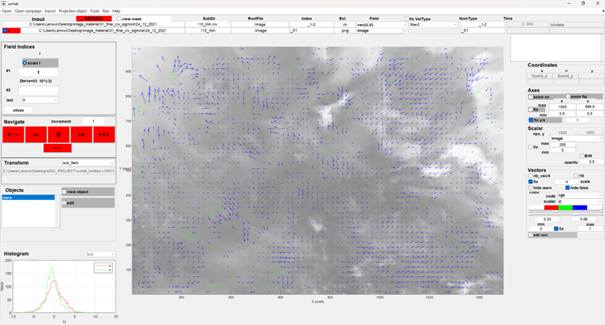
\includegraphics[width=1\textwidth]{fig_28.png}
    \caption{Screenshot of the UVMAT interface used for performing CIV\cite{SoftUVMAT}.}
\end{figure}
\FloatBarrier
The parameters (see Figure 3.10), were set based on visual observations and cloud features sizes. 
The interrogation window size was chosen to be sufficiently large to maximize detection probability while avoiding excessive size that could lead to mismatches. Similarly, the shift box was sized to match small cloud features to ensure efficient movement detection. Ideally, the correlation box should be kept as small as possible; however, if too small, there are insufficient pixels for accurate matching, leading to reduced correlation and an increase in false vectors.

The grid size should also match the size of the correlation area: a smaller grid leads to oversampling, whereas a larger grid provides too few vectors. In this instance, a slightly smaller grid size was defined to enhance result visualization by increasing vector density.

Additionally, the choice of time interval is important. A longer time interval can yield more accurate velocity vector measurements. However, if the interval is excessively long, cloud deformation over time renders the movements undetectable.
\FloatBarrier
\begin{figure}[h!] 
    \centering
    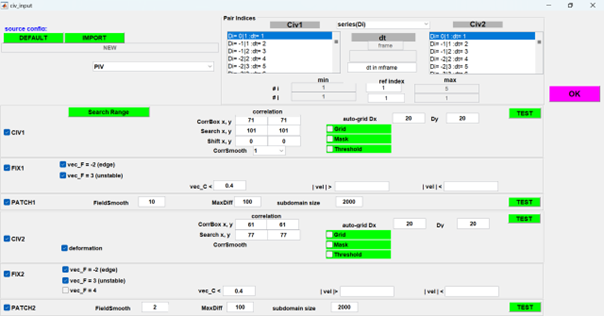
\includegraphics[width=1\textwidth]{fig_29.png}
    \caption{Screenshot of the CIV parameters used in this thesis.}
\end{figure}
\FloatBarrier
\subsection{Velocity Field Extraction}

To extract velocity fields, the results from CIV were imported into Python. The data was converted from pixel coordinates (x and y) to longitude and latitude, and from the zonal (u) and meridional (v) components, measured in pixels per time unit, to meters per second. The magnitude was calculated by determining the Euclidean distance between the u and v components, divided by the time interval. 

The transformation of CIV \( x\) and \( y\) coordinates into longitude and latitude in degrees was performed using the following formulas\cite{AlBlooki2023}: 

\begin{equation}
lon = \lambda_w + (\lambda_e - \lambda_w) \cdot \frac{x_{\text{civ}}}{n_x}
\end{equation}

\begin{equation}
lat = \phi_n + (\phi_s - \phi_n) \cdot \frac{y_{\text{civ}}}{n_y}
\end{equation}

\( \lambda_e\) and \( \lambda_w\) denote the eastern and western limits of the longitude grid, while \( \phi_n\) and \( \phi_s\) represent the northern and southern limits of the latitude grid. \( n_x\) indicates the total number of pixels along the x-axis, and \( n_y\) represents the total number of pixels along the y-axis.

The conversion of pixel per time separation to \( m s^-1\) was done as follows:
\begin{equation}
u = \frac{u_{\text{civ}}}{\triangle t} \cdot \frac{\lambda_e - \lambda_w}{\triangle x} \cdot \frac{\pi}{180} \cdot r \cdot \cos(\phi)
\end{equation}

\begin{equation}
v = \frac{v_{\text{civ}}}{\triangle t} \cdot \frac{\phi_n - \phi_s}{\triangle y} \cdot \frac{\pi}{180} \cdot r
\end{equation}

Where \( \triangle t\) is 600 or 1800 depending on the image sequence, \( \triangle x\) = \( \triangle y\) is 0.0625°/pixel,  \( \phi_n\) and \( \phi_s\) are the planetocentric latitudes and \( r\) is the radius of Mars (3389500 meters). \( \cos(\phi)\) is the cosine of the latitude factor, included to account for the variation in latitudinal distance. Figure 3.11 illustrates the geometric and trigonometric relationships that form the basis for the properties of latitude and longitude.
\FloatBarrier
\begin{figure}[h!] 
    \centering
    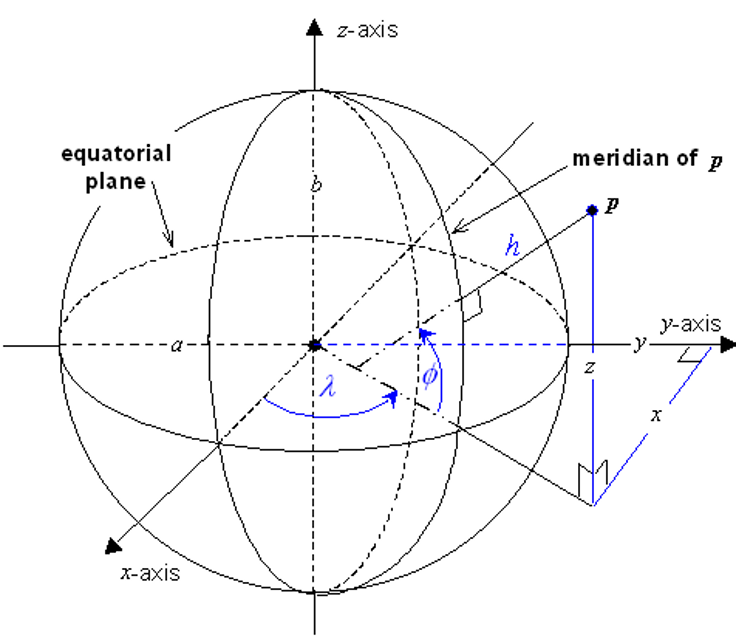
\includegraphics[width=0.8\textwidth]{fig_30.png}
    \caption{Illustration of the geodetic coordinate system geometric and trigonometric relationships\cite{ISO18026}.}
\end{figure}
\FloatBarrier